\begin{figure}[htbp]
\centering
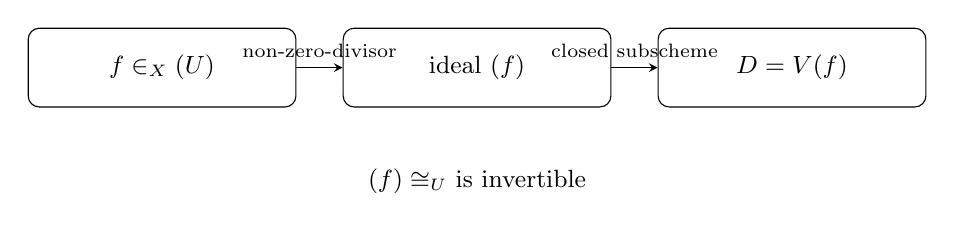
\begin{tikzpicture}[>=stealth,every node/.style={font=\small}]
\node[draw,rounded corners,minimum width=3.4cm,minimum height=1cm] (f) at (-4,0) {$f\in\OO_X(U)$};
\node[draw,rounded corners,minimum width=3.4cm,minimum height=1cm] (i) at (0,0) {ideal $(f)$};
\node[draw,rounded corners,minimum width=3.4cm,minimum height=1cm] (d) at (4,0) {$D=V(f)$};
\draw[->] (f)--node[above,font=\scriptsize]{non-zero-divisor}(i);
\draw[->] (i)--node[above,font=\scriptsize]{closed subscheme}(d);
\node at (0,-1.45) {$(f)\cong\OO_U$ is invertible};
\end{tikzpicture}
\caption{An effective Cartier divisor is locally principal in the strong sense: its local generator is a non-zero-divisor.}
\label{fig:vi40-effective}
\end{figure}
